\documentclass[10pt]{beamer}
\usetheme[background=light,block=fill,progressbar=foot]{metropolis}

%% ctex configuration. slow compiling, comment unless using Chinese.
\usepackage[UTF8]{ctex}
\ctexset{refname=References}
\ctexset{figurename=Fig.}
%%

\usepackage{graphicx}
\usepackage{caption}
\usepackage{bm}
\usepackage{booktabs}
\usepackage{natbib}
\usepackage{algorithm}
\usepackage{algorithmic} 
\usepackage{transparent}
\newcommand{\supercite}[1]{\textsuperscript{\textsuperscript{\cite{#1}}}}
\newcommand{\emoji}[1]{\text{\raisebox{-0.2em}{\includegraphics[height=1em]{emojis/#1.png}}}}

\begin{document}
	\title{Deep Learning Book}
	\subtitle{Chapter 7 \\ Regularization for Deep Learning}
	\author{Botian Shi \\ botianshi@bit.edu.cn}
	\date{March 14, 2017}
	
	\setbeamercovered{transparent=15}
	
	\begin{frame}[plain]
		\titlepage
	\end{frame}
	
	\begin{frame}
		You can download the \LaTeX\, source code of this file from \href{https://github.com/friskit-china/DLBookSlides}{\underline{Here}}.
	\end{frame}
	
	\begin{frame}{Generalization and Strategy}
		\begin{itemize}
			\item How to make an algorithm that will perform well not just on the training data, but also on new inputs? (Generalization)
			\pause
			\item Many strategies designed to reduce the test error, possibly at the expense of increased training error.
			\pause
			\item These strategies are known collectively as \textbf{regularization}.
			\pause
			\item Many regularization algorithm have been developed.
			\pause
			\item Developing more effective regularization strategies is one of the major research efforts in the field.
			\pause
			\item In this chapter, we describe regularization in more detail, focusing on regularization strategies for deep models or models that may be used as building blocks to form deep models.
		\end{itemize}
	\end{frame}
	
	\begin{frame}{Generalization and Strategy}
		\begin{itemize}
			\item There are many regularization strategies.
			\begin{enumerate}
				\pause
				\item Put extra constrains on a machine learning model. (Adding restrictions on the parameter values.)
				\pause
				\item Add extra terms in the objective function that can be thought of as corresponding to a soft constraint on the parameter values.
			\end{enumerate}
			\pause
			\item If chosen carefully, these extra constraints and penalties can lead to improved performance on the test set.
			\pause
			\item Sometimes these constraints and penalties are designed to
			\begin{enumerate}
				\item \textbf{encode} specific kinds of \textbf{prior knowledge}.
				\item express a generic preference for a simpler model class in order to promote generalization.
				\item make an under-determined problem determined. (Provide more information)
			\end{enumerate}
			\pause
			\item Other forms of regularization, known as ensemble methods, combine multiple hypotheses that explain the training data.
		\end{itemize}
	\end{frame}
	
	\begin{frame}{Generalization and Strategy}
		\begin{itemize}
			\item Principle: Treading increased bias for reduced variance.
			\pause
			\item An effective regularizer is one that makes a profitable trade, \textbf{reducing variance} significantly while not overly \textbf{increasing the bias}.
			\pause
			\item In practice, \textbf{an overly complex model family does not necessarily include the target function or the true data generating process, or even a close approximation}.
			\pause
			\item We almost never have access to the true data generating process so we can never know for sure \textbf{if the model family being estimated includes the generating process or not}.		
		\end{itemize}
	\end{frame}

	\begin{frame}{Generalization and Strategy}
		\begin{itemize}
			\item However, most applications of deep learning algorithms are to domains where the true data generating process is almost certainly outside the model family.
			\pause
			\item Deep learning algorithms are typically applied to \textbf{extremely complicated domains} such as images, audio sequences and text, for which the true generation process essentially involves \textbf{simulating the entire universe}.
			\pause
			\item To some extent, we are always trying to fit a square peg(the data generating process) into a round hole (our model family)\\ 『持方枘(ruì)而欲内圆凿』.
			\pause
			\item What this means is that controlling the complexity of the model is not a simple matter of finding the model of the \textbf{right size}, with the \textbf{right number of parameters}.
			\pause
			\item Instead, we might find that the best fitting model is a large model that has been regularized appropriately.
			\pause
			\item We now review several strategies for how to create such a large, deep, regularized model.
		\end{itemize}
	\end{frame}
	
	\begin{frame}{Parameter Norm Penalties}
		\begin{itemize}
			\pause
			\item Regularization has been used for decades prior to the advent of deep learning.
			\pause
			\item Linear models allow simple straightforward and effective regularization strategies.
			\pause
			\item Most approaches are based on limiting the capacity of models by adding a \textbf{parameter norm penalty} $\Omega(\theta)$ to the objective function $J$:
			$$\tilde{\mathit{J}}(\bm{\theta};\bm{X},\bm{y})=\mathit{J}(\bm{\theta};\bm{X},\bm{y})+\alpha\Omega(\bm{\theta})$$
			where $\alpha\in[0,+\infty)$ weights the relative contribution of the norm penalty term.
			\pause
			\item Setting $\alpha$ to 0 results in no regularization. Larger values of $\alpha$ correspond to more regularization.
			\pause
			\item Optimize both $J$ and norm
			\pause
			\item Different $\Omega$ has different result.
		\end{itemize}
	\end{frame}
	
	\begin{frame}{Parameter Norm Penalties}
		\begin{itemize}
			\item We penalize \textbf{only the weights} of the affine transformation at each layer and leaves the biases unregularized.
			\pause
			\item We do not induce too much variance by leaving the biases unregularized.
			\pause
			\item Regularizing the bias parameters can introduce a significant amount of under-fitting.
			\pause
			\item We therefore use the vector $\bm{w}$ to indicate all of the weights that should be affected by a norm penalty, while the vector $\bm{\theta}$ denotes all of the parameters, including both $\bm{w}$ and the unregularized parameters.
			\pause
			\item Sometime we use a separate penalty with a different $\alpha$ coefficient for each layer.
			\pause
			\item But it can be expensive to search for the correct value of multiple hyper-parameters, it is still reasonable to use the same weight decay at all layers just to reduce the size of search space.
		\end{itemize}
	\end{frame}
	
	\begin{frame}{$L^2$ Parameter Regularization}
		\begin{itemize}
			\pause
			\item The $L^2$ norm penalty commonly known as \emph{weight decay}.
			\pause
			$$\Omega(\bm{\theta})=\frac{1}{2}\lVert w\rVert^2_2$$
			
			\pause
			\item This regularization strategy drives the weights closer to the origin. (as well as \emph{ridge regression} or \emph{Tikhonov regularization})
			\pause
			\item We can gain some insight into the behavior of weight decay regularization. (assume no bias for simplification)
			$$\tilde{J}(\bm{w};\bm{X},\bm{y})=\frac{\alpha}{2}\bm{w}^T\bm{w}+J(\bm{w};\bm{X},\bm{y})$$
			$$\nabla_{\bm{w}}\tilde{J}(\bm{w};\bm{X},\bm{y})=\alpha\bm{w}+\nabla_{\bm{w}}J(\bm{w};\bm{X},\bm{y})$$
			
			\pause
			\item The update
			$$\bm{w}\leftarrow\bm{w}-\epsilon(\alpha\bm{w}+\nabla_{\bm{w}}J(\bm{w};\bm{X},\bm{y}))$$
			$$\bm{w}\leftarrow(1-\epsilon\alpha)\bm{w}-\epsilon\nabla_{\bm{w}}J(\bm{w};\bm{X},\bm{y})$$

			\pause
			\item Shrink the weight vector by a constant factor on each step.
			\pause
			\item What happens over the entire course of training?
		\end{itemize}
	\end{frame}
	
	\begin{frame}{Recall: Quadratic Approximation}
		\begin{itemize}
			\pause
			\item In mathematics, approximation theory is concerned with how functions can best be approximated with simpler functions.
			\pause
			\item \textbf{local linear approximation} and \textbf{taylor expansion}
			\begin{enumerate}
				\pause
				\item For example, when the independent variable of function $y=x^3$ changes, which is $\Delta x$, the variation of $y$ is
				$$\Delta y=(x+\Delta x)^3-x^3=3x^2\Delta x+3x(\Delta x)^2+(\Delta x)^3$$
				
				\pause
				\item When $\Delta x\rightarrow0$, omit last two terms: $\Delta y=3x^2\Delta x$
				\pause
				\item In general:
				$$\Delta y=f(x_0+\Delta x)-f(x_0)\approx f'(x_0)\times\Delta x$$
				$$\Delta y=f(x)-f(x_0)\text{,~}\Delta x=x-x_0$$
				$$f(x)-f(x_0)=f'(x_0)\times(x-x_0)$$
				$$f(x)=f(x_0)+f'(x_0)(x-x_0)$$
				
				\pause
				\item In order to improve the precision, we can use second-order approximation, which is the second-order Taylor series expansion.
				$$f(x)=f(x_0)+\frac{f'(x_0)}{1!}(x-x_0)+\frac{f''(x_0)}{2!}(x-x_0)^2$$
			\end{enumerate}
		\end{itemize}
	\end{frame}

	\begin{frame}{$L^2$ Parameter Regularization}
		\begin{itemize}
			\pause
			\item Let $\bm{w}^*=\arg\min_{\bm{w}}J(\bm{w})$ (unregularized training cost)
			\pause
			\item Making a quadratic approximation to the objective function in the neighborhood of the value of the weights. (In DLBook, they used $\hat{J}(\bm{\theta})$, but here we use $\hat{J}(\bm{w})$ to explain easier)
			$$\hat{\bm{J}}(\bm{w})=\bm{J}(\bm{w}^*)+\frac{1}{2}(\bm{w}-\bm{w}^*)^T\bm{\mathbf{H}}(\bm{w}-\bm{w}^*)$$
			\item Where $\mathbf{H}$ is the Hessian matrix of $J$ with respect to $\bm{w}$ evaluated at $\bm{w}^*$.
			\pause
			\item There is no first-order term in this quadratic approximation, because $\bm{w}^*$ is defined to be a minimum, where the gradient vanishes.
			\pause
			\item The minimum of $\hat{J}$ occurs where its gradient
			$$\nabla_{\bm{w}}\hat{\bm{J}}(\bm{w})=\mathbf{H}(\bm{w}-\bm{w}^*)$$
			is equal to 0.
		\end{itemize}
	\end{frame}
	
	\begin{frame}{$L^2$ Parameter Regularization}
		\begin{itemize}
			\item To study the effect of weight decay, we modify $\nabla_{\bm{w}}\hat{\bm{J}}(\bm{w})=\mathbf{H}(\bm{w}-\bm{w}^*)$ by adding the weight decay gradient.
			\pause
			\item We can solve for the minimum of the regularized version of $\hat{\bm{J}}$.
			\item We use the variable $\tilde{\bm{w}}$ to represent the location of the minimum.
			$$\alpha\tilde{\bm{w}}+\mathbf{H}(\tilde{\bm{w}}-\bm{w}^*)=0$$
			$$(\mathbf{H}+\alpha\mathbf{I})\tilde{\bm{w}}=\mathbf{H}\bm{w}^*$$
			$$\tilde{\bm{w}}=\frac{\mathbf{H}\bm{w}^*}{(\mathbf{H+\alpha\mathbf{I}})}$$
			
			\pause
			\item As $\alpha$ approaches 0, the regularized solution $\tilde{\bm{w}}$ approaches $\bm{w}^*$.
			\item But what happens as $\alpha$ grows?
		\end{itemize}
	\end{frame}
	
	\begin{frame}{$L^2$ Parameter Regularization}
		\begin{itemize}
			\item Because $\mathbf{H}$ is real and symmetric, we can decompose it into a diagonal matrix $\bm{\Lambda}$ and an orthonormal basis of eigenvectors, $\bm{Q}$, such that $\mathbf{H}=\bm{Q\Lambda Q}^T$.
			\pause
			\item Applying the decomposition $\tilde{\bm{w}}=(\mathbf{H+\alpha\mathbf{I}})^{-1}\mathbf{H}\bm{w}^*$
			\begin{eqnarray*}
				\tilde{\bm{w}}&=&(\bm{Q\Lambda Q}^T+\alpha\bm{I})^{-1}\bm{Q\Lambda Q}^T\bm{w}^*\\
				&=&\left[\bm{Q}(\bm{\Lambda}+\alpha\bm{I})\bm{Q}^T\right]^{-1}\bm{Q\Lambda Q}^T\bm{w}^*\\
				&=&\bm{Q}(\bm{\Lambda}+\alpha\bm{I})^{-1}\bm{\Lambda Q}^T\bm{w}^*\\
				&=&\bm{Q}\frac{\bm{\Lambda}}{\bm{\Lambda}+\alpha\bm{I}}\bm{Q}^T\bm{w}^*
			\end{eqnarray*}
			\pause
			\item We see that the effect of weight decay is to rescale $\bm{w}^*$ along the axes defined by the eigenvectors of $\bm{H}$.
			\pause
			\item Specifically, the component of $\bm{w}^*$ that is aligned with the $i$-th eigenvector of $\bm{H}$ is rescaled by a factor of $\frac{\lambda_i}{\lambda_i+\alpha}$
		\end{itemize}
	\end{frame}

	\begin{frame}{$L^2$ Parameter Regularization}
		This effect is illustrated in figure:
		\begin{figure}
			\caption{An illustration of the effect of $L^2$ (or weight decay) regularization on the value of the optimal $\bm{w}$}
			\vspace{-1em}
			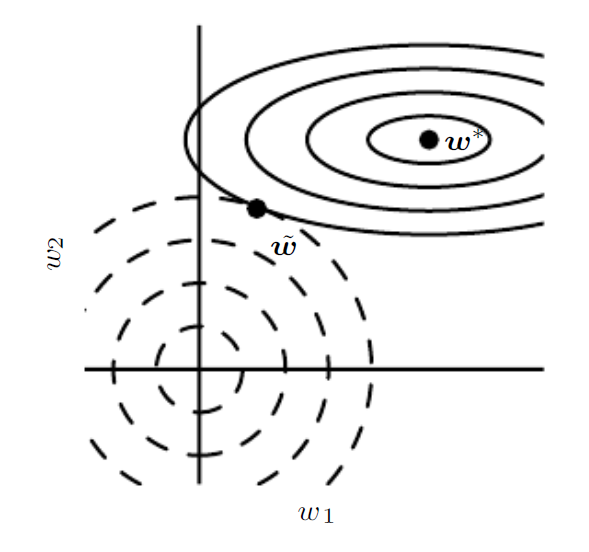
\includegraphics[height=10em]{figures/l2-regularization.png}
			\vspace{-1em}
		\end{figure}
		\begin{itemize}
			\pause
			\item The solid ellipses represent contours of equal value of the \textbf{unregularized objective}.
			\pause
			\item The dotted circles represent contours of equal value of the $L^2$ regularizer.
			\pause
			\item At the point $\tilde{\bm{w}}$, these competing objectives reach an equilibrium.
		\end{itemize}
	\end{frame}
	
	\begin{frame}{$L^2$ Parameter Regularization}
		\begin{figure}
			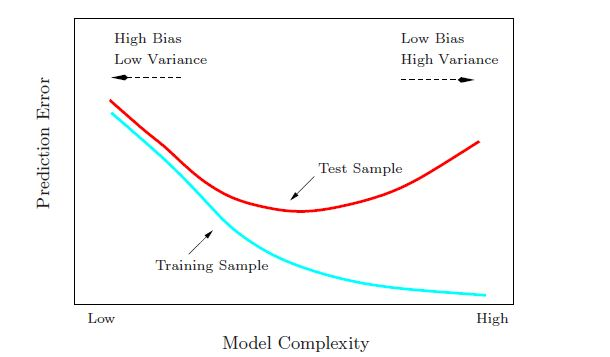
\includegraphics[height=15em]{figures/bias-variance.jpg}
		\end{figure}
	\end{frame}

	\begin{frame}{$L^2$ Parameter Regularization}
		\begin{itemize}
			\item How do these effects relate to machine learning in particular?
			\pause
			\item We can find out by studying linear regression, the cost function is the sum of squared errors:
			$$(\bm{Xw}-\bm{y})^T(\bm{Xw}-\bm{y})$$
			
			\pause
			\item Add $L^2$ regularization, the objective function changes to:
			$$(\bm{Xw}-\bm{y})^T(\bm{Xw}-\bm{y})+\frac{1}{2}\alpha\bm{w}^T\bm{w}$$
			
			\pause
			\item This changes the normal equations for the solution from:
			$$\bm{w}=(\bm{X}^T\bm{X})^{-1}\bm{X}^T\bm{y} \text{~to~} \bm{w}=(\bm{X}^T\bm{X}+\alpha\bm{I})^{-1}\bm{X}^T\bm{y}$$
			
			\pause
			\item The new matrix has the addition of $\alpha$ to the diagonal.
			\pause
			\item Diagonal correspond to the variance of each input feature.
			\pause
			\item We can see that $L^2$ regularization causes the learning algorithm to "perceive" the input $\bm{X}$ as having higher variance, which makes it shrink the weights on features whose covariance with the output target is low compared to this added variance.
		\end{itemize}
	\end{frame}

	\begin{frame}{$L^1$ Regularization}
		\begin{itemize}
			\item $L^1$ regularization on the model parameter $w$ is defined as:
			$$\Omega(\bm{\theta})=\lVert\bm{w}\rVert_1=\sum_i\left|w_i\right|$$
			
			\item We will now discuss the effect of $L^1$ regularization on the simple linear regression model, with no bias parameters, that we studied in our analysis of $L^2$ regularization.
			\pause
			\item In particular, we are interested in delineating the differences between $L^1$ and $L^2$ forms of regularization.
		\end{itemize}
	\end{frame}

	\begin{frame}{$L^1$ Regularization}
		\begin{itemize}
			\item As with $L^2$ weight decay, $L^1$ weight decay controls the strength of the regularization by scaling the penalty $\Omega$ using a positive hyperparameter $\alpha$.
			\pause
			\item Thus, the regularized objective function $\tilde{J}(\bm{w};\bm{X},\bm{y})$ is given by
			$$\tilde{J}(\bm{w};\bm{X},\bm{y})=\alpha\lVert\bm{w}\rVert_1+J(\bm{w;\bm{X},\bm{y}})$$
			
			\pause
			with the corresponding gradient:
			$$\nabla_{\bm{w}}\tilde{J}(\bm{w};\bm{X},\bm{y})=\alpha\mathrm{sign}(\bm{w})+\nabla_{\bm{w}}J(\bm{w};\bm{X},\bm{y})$$
			
			\pause
			where $\mathrm{sign}(\bm{w})$ is simply the sign of $\bm{w}$ applied element-wise.
			
		\end{itemize}
	\end{frame}

	\begin{frame}{$L^1$ Regularization}
		$$\nabla_{\bm{w}}\tilde{J}(\bm{w};\bm{X},\bm{y})=\alpha\mathrm{sign}(\bm{w})+\nabla_{\bm{w}}J(\bm{w};\bm{X},\bm{y})$$
		\begin{itemize}
			\item From this equation, we can see that the effect of $L^1$ regularization is quite different from that of $L^2$ regularization.
			\pause
			\item We can see that the regularization contribution to the gradient no longer scales linearly with each $w_i$; instead it is a constant factor with a sign equal to $\mathrm{sign}(w_i)$.
			\pause
			\item One consequence of this form of the gradient is that we will not necessarily see clean algebraic solutions to quadratic approximations of $J(\bm{X},\bm{y};\bm{w})$ as we did for $L^2$ regularization.
		\end{itemize}
	\end{frame}
	
	\begin{frame}{$L^1$ Regularization}
		\begin{itemize}
			\item Out simple linear model has a quadratic cost function that we can represent via its Taylor series.
			\pause
			\item Alternately, we could imaging that this is a truncated Taylor series approximating the cost function of a more sophisticated model. 
			\pause
			\item The gradient in this setting is given by
			$$\nabla_w\tilde{J}(\bm{w})=\mathbf{H}(\bm{w}-\bm{w}^*)$$
			
			\pause
			\item Because the $L^1$ penalty does not admit clean algebraic expressions in the case of a full general Hessian, we will also make the further simplifying assumption that the Hessian is a diagonal, $\mathbf{H}=\mathrm{diag}([H_{1,1},\dots,H_{n,n}])$, where each $H_{i,i}>0$.
			\pause
			\item This assumption holds if the data for the linear regression problem has been preprocessed to remove all correlation between the input features, which may be accomplished using PCA.
		\end{itemize}
	\end{frame}

	\begin{frame}{$L^1$ Regularization}
		\begin{itemize}
			\item Our quadratic approximation of the $L^1$ regularized objective function decomposes into a sum over the parameters:
			$$\tilde{J}(\bm{w};\bm{X},\bm{y})=J(\bm{w}^*;\bm{X},\bm{y})+\sum_i\left[\frac{1}{2}H_{i,i}(\bm{w}_i-\bm{w}_i^*)^2+\alpha\left|w_i\right|\right]$$
			
			\pause
			\item The problem of minimizing this approximate cost function has an analytical solution (for each dimension $i$), with the following form:
			$$w_i=\mathrm{sign}(w_i^*)max\left\{\left|w_i^*\right|-\frac{\alpha}{H_{i,i}}, 0\right\}$$
		\end{itemize}
	\end{frame}

	\begin{frame}{$L^1$ Regularization}
		$$w_i=\mathrm{sign}(w_i^*)max\left\{\left|w_i^*\right|-\frac{\alpha}{H_{i,i}}, 0\right\}$$
		
		\begin{itemize}
			\pause
			\item Consider the situation where $w_i^*>0$ for all $i$. There are two possible outcomes:
			\begin{enumerate}
				\pause
				\item The case where $w_i^*\leq\frac{\alpha}{H_{i,i}}$. Here the optimal value of $w_i$ under the regularized objective is simply $w_i=0$. This occurs because the contribution of $J(\bm{w};\bm{X},\bm{y})$ to the regularized objective $\tilde{J}(\bm{w};\bm{X},\bm{y})$ is overwhelmed--in direction $i$--by the $L^1$ regularization which pushes the value of $w_i$ to zero.
				\pause
				\item The case where $w_i^*>\frac{\alpha}{H_{i,i}}$. In this case, the regularization does not move the optimal value of $w_i$ to zero but instead it just shifts it in that direction by a distance equal to $\frac{\alpha}{H_{i,i}}$.
			\end{enumerate}
			\pause
			\item A similar process happens when $w_i^*<0$, but with the $L^1$ penalty making $w_i$ less negative by $\frac{\alpha}{H_{i,i}}$, or 0.
		\end{itemize}
	\end{frame}

	\begin{frame}{$L^1$ Regularization}
		\begin{itemize}
			\item In comparison to $L^2$ regularization, $L^1$ regularization results in a solution that is more \emph{sparse}.
			\pause
			\item Sparsity in this context refers to the fact that some parameters have an optimal value of zero.
			\pause
			\item The sparsity property induced by $L^1$ regularization has been used extensively as a \emph{feature selection} mechanism.
			\pause
			\item Feature selection simplifies a machine learning problem by choosing which subset of the available features should be used.
			\pause
			\item In particular, the well known LASSO (\citep{tibshirani1996regression}) (least absolute shrinkage and selection operator) model integrates an $L^1$ penalty with a linear model and a least squares cost function.
		\end{itemize}
	\end{frame}

	\begin{frame}{Sparsity? $L^1$ and $L^2$}
		\begin{figure}
			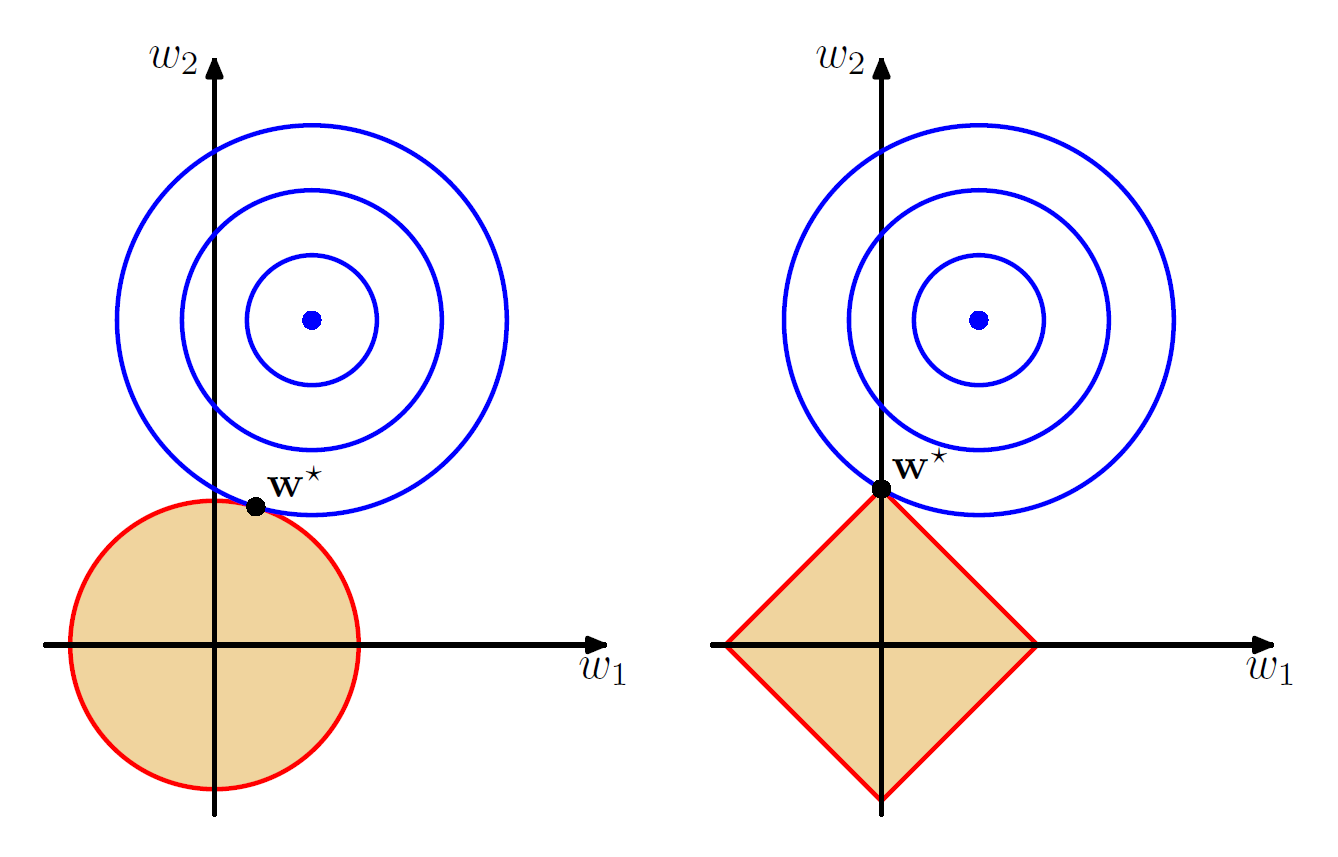
\includegraphics[height=15em]{figures/prml-l1-l2-contours.png}
			\caption{Plot of the contours of the unregularized error function (blue) along with the constraint region for the quadratic regularizer on the left and the lasso regularizer on the right.}
		\end{figure}
	\end{frame}
	
	\begin{frame}{Norm Penalties as Constrained Optimization}
		\begin{itemize}
			\item Consider the cost function regularized by a parameter norm penalty:
			$$\tilde{J}(\bm{\theta};\bm{X},\bm{y})=J(\bm{\theta};\bm{X},\bm{y})+\alpha\Omega(\bm{\theta})$$
			
			\pause
			\item If we want to constrain $\Omega(\bm{\theta})$ to be less than some constant $k$, we could construct a generalized Lagrange function
			$$\mathcal{L}(\bm{\theta,\alpha;\bm{X},\bm{y}})=J(\bm{\theta};\bm{X},\bm{y})+\alpha(\Omega(\theta)-k)$$
			
			\pause
			\item The solution to the constrained problem is given by
			$$\bm{\theta}^*=\mathop{\arg\min}_{\bm{\theta}}\mathop{\max}_{\alpha,\alpha\geq0}\mathcal{L}(\bm{\theta,\alpha}) $$
		\end{itemize}
	\end{frame}

	\begin{frame}{Norm Penalties as Constrained Optimization}
		$$\bm{\theta}^*=\mathop{\arg\min}_{\bm{\theta}}\mathop{\max}_{\alpha,\alpha\geq0}\mathcal{L}(\bm{\theta,\alpha}) $$
		
		\begin{itemize}
			\item Solving this problem requires modifying both $\bm{\theta}$ and $\alpha$.
			\pause
			\item Many different procedures are possible--some may use gradient descent, while others may use analytical solutions for where the gradient is zero--but in all procedures $\alpha$ must increase whenever $\Omega(\bm{\theta})>k$ and decrease whenever $\Omega(\bm{\theta})<k$.
			\pause
			\item All positive $\alpha$ encourage $\Omega(\bm{\theta})$ to shrink.
			\pause
			\item The optimal value $a^*$ will encourage $\Omega(\theta)$ to shrink, but not so strongly to make $\Omega(\bm{\theta})$ become less than $k$.
		\end{itemize}
	\end{frame}
	
	\begin{frame}{Norm Penalties as Constrained Optimization}
		\begin{itemize}
			\item To gain some insight into the effect of the constraint, we can fix $\alpha^*$ and view the problem as just a function of $\theta$:
			$$\bm{\theta}^*=\mathop{\arg\min}_{\bm{\theta}}\mathcal{L}(\bm{\theta}, \alpha^*)=\mathop{\arg\min}_{\bm{\theta}}J(\bm{\theta};\bm{X},\bm{y})+\alpha*\Omega(\bm{\theta})$$
			
			\item This is exactly the same as the regularized training problem of minimizing $\tilde{J}$.
			
			\pause
			\item We can thus think of a parameter norm penalty as imposing a constraint on the weights.
			\pause
			\item If $\Omega$ is the $L^2$ norm, then the weights are constrained to lie in an $L^2$ ball.
			\pause
			\item If $\Omega$ is the $L^1$ norm, then the weights are constrained to lie in a region of limited $L^1$ norm.
			
		\end{itemize}
	\end{frame}

	\begin{frame}{Regularization and Under-Constrained Problems}
		\begin{itemize}
			\item In some cases, regularization is necessary.
			\pause
			\item Many linear models in machine learning, including linear regression and PCA, depend on inverting the matrix $\bm{X}^T\bm{X}$.
			\pause
			\item This is not possible whenever $\bm{X}^T\bm{X}$ is singular.
			\pause
			\item This matrix can be singular whenever the data generating distribution truly has no variance in some direction, or when no variance in \textbf{observed} in some direction because there are fewer examples (rows of $\bm{X}$) than input features (columns of $\bm{X}$).
			\pause
			\item In this case, many forms of regularization correspond to inverting $\bm{X}^T\bm{X}+\alpha\bm{I}$ instead. This regularized matrix is guaranteed to be invertible.
		\end{itemize}
	\end{frame}

	\begin{frame}{Regularization and Under-Constrained Problems}
		\begin{itemize}
			\item These linear problems have closed form solutions when the relevant matrix is invertible. 
			\pause
			\item It is also possible for a problem with no closed form solution to be underdetermined.
			\pause
			\item An example is logistic regression applied to a problem where the classes are linearly separable.
			\pause
			\item If a weight vector $\bm{w}$ is able to achieve perfect classification, then $2\bm{w}$ will also achieve perfect classification and higher likelihood.
			\pause
			\item An iterative optimization procedure like SGD will continually increase the magnitude of $\bm{w}$ and, in theory, will never halt.
			\pause
			\item Most forms of regularization are able to guarantee the convergence of iterative methods applied to underdetermined problems.
			\pause
			\item For example, weight decay will cause gradient descent to quit increasing the magnitude of the weights when the slope of the likelihood is equal to the weight decay coefficient.
		\end{itemize}
	\end{frame}
	
	\begin{frame}{Regularization and Under-Constrained Problems}
		\begin{itemize}
			\item We can solve underdetermined linear equations using the Moore-Penrose pseudoinverse. Recall that one definition of the pseudoinverse $\bm{X}^+$ of a matrix $\bm{X}$ is
			$$\bm{X^+}=\lim_{a\rightarrow0}(\bm{X}^T\bm{X}+\alpha\bm{I})^{-1}\bm{X}^T$$
			
			\pause
			\item We can now recognize this equation as performing linear regression with weight decay.
			\pause
			\item We can interpret the pseudoinverse as stabilizing underdetermined problems using regularization.
		\end{itemize}
	\end{frame}

	\begin{frame}{Dataset Augmentation}
		\begin{itemize}
			\pause
			\item The best way to make a machine learning model generalize better is to train it on more data.
			\pause
			\item In practice, the amount of data we have is limited.
			\pause
			\item Create fake data and add it to the training set.
			\pause
			\item This approach is easiest for classification.
			\pause
			\item A classifier needs to take a complicated, high dimensional input $\bm{x}$ and summarize it with a single category identity $y$.
			\pause
			\item This means that the main task facing a classifier is to be invariant to a wide variety of transformations.
			\pause
			\item We can generate new $(\bm{x},y)$ pairs easily just by transforming the $\bm{x}$ inputs in our training set.
		\end{itemize}
	\end{frame}

	\begin{frame}{Dataset Augmentation}
		\begin{itemize}
			\item Dataset augmentation has been a particularly effective technique for a specific classification problem: object recognition.
			\pause
			\item Images are high dimensional and include an enormous variety of factors of variation, many of which can be easily simulated.
			\pause
			\item One must be careful not to apply transformations that would change the correct class. (e.g. '6' and '9', 'b' and 'd').
		\end{itemize}
	\end{frame}

	\begin{frame}{Dataset Augmentation}
		\begin{itemize}
			\item Dataset augmentation is effective for speech recognition task as well (\citet{jaitly2013vocal}).
			\pause
			\item Inject noise in the input to a neural network can also be seen as a form of data augmentation (\citet{sietsma1991creating}).
			\pause
			\item For many classification and even some regression tasks, the task should still be possible to solve even if small random noise is added to the input.
			\pause
			\item One way to improve the robustness of neural networks is simply to train them with random noise applied to their inputs.
			\pause
			\item Input noise injection is part of some unsupervised learning algorithms such as the denoising autoencoder (\citet{vincent2008extracting}).
			\pause
			\item Dropout, a powerful regularization strategy can be seen as a process of constructing new inputs by \textbf{multiplying} by noise.
		\end{itemize}
	\end{frame}

	\begin{frame}{Dataset Augmentation}
		\begin{itemize}
			\item When comparing machine learning benchmark results, it is important to take the effect of dataset augmentation into account.
			\pause
			\item Often, hand-designed dataset augmentation schemes can dramatically reduce the generalization error.
			\pause
			\item When comparing machine learning algorithm A and machine learning algorithm B, it is necessary to make sure that both algorithms were evaluated using the same hand-designed dataset augmentation schemes.
		\end{itemize}
	\end{frame}

	\begin{frame}{Noise Robustness}
		\begin{itemize}
			\item For some models, the addition of noise with infinitesimal variance at the input of the model is equivalent to imposing a penalty on the norm of the weights (\citet{bishop1995regularization,bishop1995training}).
			\pause
			\item Noise injection can be much more powerful than simply shrinking the parameters, especially when the noise is added to the hidden units.
			\pause
			\item Noise applied to the hidden units is such an important topic; the dropout algorithm describe later.
			\pause
			\item Another way that noise can be added into the weights.
			\pause
			\item This technique has been used primarily in the context of recurrent neural networks (\citet{jim1996analysis,graves2011practical}).
			\pause
			\item This can also be interpreted as equivalent (under some assumptions) to a more traditional form of regularization.
		\end{itemize}
	\end{frame}

	\begin{frame}{Noise Robustness}
		\begin{itemize}
			\item We study the regression setting, where we wish to train a function $\tilde{y}(\bm{x})$ that maps a set of features $\bm{x}$ to a scalar using the least-squares cost function between the model predictions $\tilde{y}(\bm{x})$ and the true values $y$:
			$$J=\mathbb{E}_{p(x,y)}\left[(\hat{y}(x)-y)^2\right]$$
			
			\pause
			\item The training set with $m$ examples: ${(\bm{x}^{(1)},y^{(1)}),\dots,(\bm{x}^{(m)},y^{(m)})}$.
			\pause
			\item We now assume that with each input presentation we also include a random perturbation $\epsilon_{\bm{W}}~\mathcal{N}(\bm{\epsilon};\bm{0},\eta\bm{I})$ of the network weights.
			\pause
			\item We denote the perturbed model as $\hat{y}_{\epsilon_{\bm{W}}}(\bm{x})$. The objective function thus becomes:
			\begin{eqnarray*}
				\tilde{J}_{\bm{W}}&=&\mathbb{E}_{p(\bm{x},y,\epsilon_{\bm{W}})}\left[(\hat{y}_{\epsilon_{\bm{w}}}(\bm{x})-y)^2\right]\\
				&=&\mathbb{E}_{p(\bm{x},y,\epsilon_{\bm{W}})}\left[\hat{y}^2_{\epsilon_{\bm{W}}}(\bm{x}-2y\hat{y}_{\epsilon_{\bm{W}}}+y^2)\right]
			\end{eqnarray*}
		\end{itemize}
	\end{frame}

	\begin{frame}{Noise Robustness}
		$$\tilde{J}_{\bm{W}}=\mathbb{E}_{p(\bm{x},y,\epsilon_{\bm{W}})}\left[\hat{y}^2_{\epsilon_{\bm{W}}}(\bm{x}-2y\hat{y}_{\epsilon_{\bm{W}}}+y^2)\right]$$
		
		\begin{itemize}
			\item For small $\eta$, the minimization of $J$ with added weight noise (with covariance $\eta\bm{I}$) is equivalent to minimization of $J$ with an additional regularization.
			\pause
			\item This form of regularization encourages the parameters to go to regions of parameter space where small perturbations of the weights have a relatively small influence on the output.
			\pause
			\item In other words, it pushes the model weights, finding points that are not merely minimal, but minimal surrounded by flat regions (\citet{hochreiter1995simplifying}).
		\end{itemize}
	\end{frame}
	
	\begin{frame}{Noise Robustness\\ Injecting Noise at the Output Target}
		\begin{itemize}
			\item Most datasets have some amount of mistakes in the $y$ labels.
			\pause
			\item It can be harmful to maximize $\log p(y|\bm{x})$ when $y$ is a mistake.
			\pause
			\item One way to prevent this is to explicitly model the noise on the labels.
			\pause
			\item For example, we can assume that for some small constant $\epsilon$, the training set label $y$ is correct with probability $1-\epsilon$, and otherwise any of the other possible labels might be correct.
		\end{itemize}
	\end{frame}

	\begin{frame}{Semi-Supervised Learning}
		\begin{itemize}
			\item In the paradigm of semi-supervised learning, both unlabeled examples from $P(\bm{x})$ and labeled examples from $P(\bm{x},\bm{y})$ are used to estimate $P(\bm{y|\bm{x}})$ or predict $\bm{y}$ from $\bm{x}$.
			\pause
			\item In the context of deep learning, semi-supervised learning usually refers to learning a representation $\bm{h=f(\bm{x})}$. The goal is to learn a representation so that \textbf{examples from the same class have similar representations}.
			\pause
			\item Unsupervised learning can provide useful cues for \textbf{how to group examples in representations space}.
			\pause
			\item Examples that cluster tightly in the input space should be mapped to similar representations.
			\pause
			\item A linear classifier in the new space may achieve better generalization in many cases.
		\end{itemize}
	\end{frame}

	\begin{frame}{Semi-Supervised Learning}
		\begin{itemize}
			\item One can construct models in which a generative model of either $(\bm{x})$ or $P(\bm{x},\bm{y})$ shares parameters with a discriminative model of $P(\bm{y}|\bm{x})$.
			\pause
			\item The generative criterion then express a particular form of prior belief about the solution to the supervised learning problem, namely that the structure of $P(\bm{x})$ is connected to the structure of $P(\bm{y}|\bm{x})$ in a way that is captured by the shared parameterization.
			\pause
			\item By controlling how much of the generative criterion is included in the total criterion, one can find a better trade-off than with a purely generative or purely discriminative training criterion.
			\pause
			\item \citet{hinton2008using} describe a method for learning the kernel function of a kernel machine used for regression, in which the usage of unlabeled examples for modeling $P(\bm{x})$ improves $P(\bm{y}|\bm{x})$ quite significantly.
		\end{itemize}
	\end{frame}
	
	\begin{frame}{Multi-Task Learning}
		\begin{itemize}
			\pause
			\item Multi-task learning is a way to improve generalization by pooling the examples arising out of several tasks.
			\pause
			\item In the same way that additional training examples put more pressure on the parameters of the model towards values that generalize well, when part of a model is shared across tasks, model often yield better generalization.
		\end{itemize}
	\end{frame}
	
	\begin{frame}{Multi-Task Learning}
		\begin{itemize}
			\item Here is a very common form of multi-task learning.
			\item Different supervised tasks (predicting $\bm{y}^{(i)}$ given $\bm{x}$) share the same input $\bm{x}$, as well as some intermediate-level representation $\bm{h}^{(\text{shared})}$ capturing a common pool of factors.
			
			\begin{columns}[T,onlytextwidth]
				\column{0.6\textwidth}
				\begin{itemize}
					\item The model has two kinds of parts:
					\begin{enumerate}
						\item Task-specific parameters (which only benefit from the examples of their task to achieve good generalization). These are the upper layers.
						\item Generic parameters, shared across all the tasks (which benefit from the pooled data of all the tasks). These are the lower years.
					\end{enumerate}
				\end{itemize}
				\column{0.4\textwidth}
				\begin{figure}
					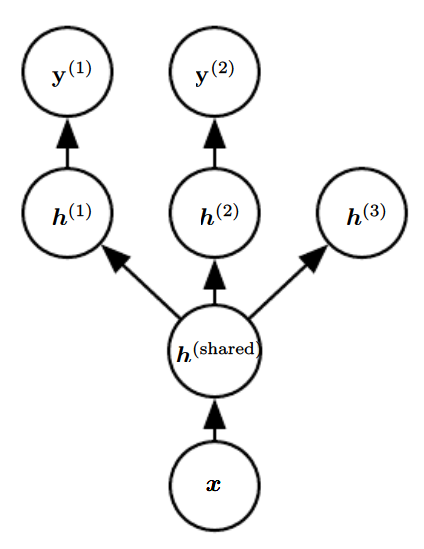
\includegraphics[height=12em]{figures/multi-task-learning.png}
				\end{figure}
			\end{columns}
			\item The factors that explain the variations are shared across two or more tasks.
		\end{itemize}
	\end{frame}

	\begin{frame}{Early Stopping}
		\begin{itemize}
			\item When training large models with sufficient representational capacity to overfit the task, we often observe that training error decreases steadily over time, but validation set error begins to rise again.
			\begin{figure}
				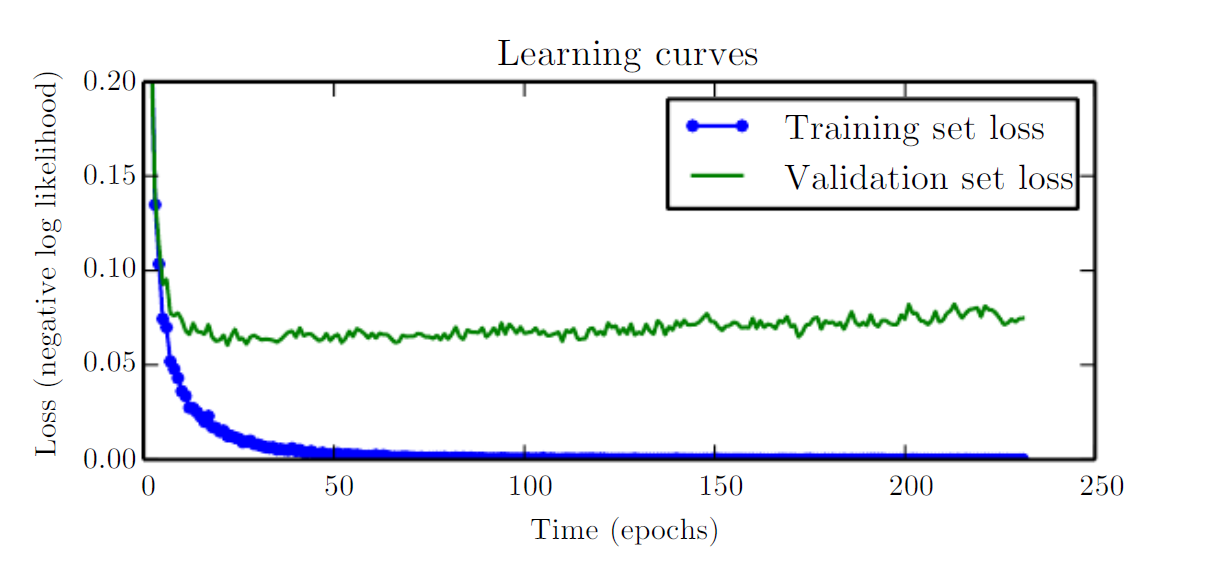
\includegraphics[height=8em]{figures/training-curve-overfit.png}
			\end{figure}
			\pause
			\item This behavior occurs very reliably.
			\pause
			\item This means we can obtain a model with better validation set error (hopefully better test set error) by returning to the parameter setting at the point in time with the lowest validation set error.
		\end{itemize}
	\end{frame}

	\begin{frame}{Early Stopping}
		\begin{itemize}
			\item Every time the error on the validation set improves, we store a copy of the model parameters.
			\pause
			\item When the training algorithm terminates, we return these parameters, rather the latest parameters.
		\end{itemize}
	\end{frame}

	\begin{frame}{Early Stopping}
		\begin{algorithm}[H]
			\caption{Early Stopping Algorithm}
			\label{alg:early-stopping}
			\begin{algorithmic}
				\pause
				\STATE Let $n$ be the number of steps between evaluations.
				\pause
				\STATE Let $p$ be the "patience", the number of times to observe worsening validation set error before giving up.
				\pause
				\STATE Let $\bm{\theta_o}$ be the initial parameters.
				\pause
				\STATE $\bm{\theta}\leftarrow\bm{\theta_o}$; $i\leftarrow0$; $j\leftarrow0$; $v\leftarrow\infty$; $i^*\leftarrow i$
				\pause
				\WHILE{$j<p$}
					\pause
					\STATE Update $\bm{\theta}$ by running the training algorithm for $n$ steps.
					\pause
					\STATE $i\leftarrow i+n$; $v'\leftarrow\text{ValidationSetError}(\bm{\theta})$
					\pause
					\IF{$v'<v$}
						\pause
						\STATE $j\leftarrow0$; $\bm{\theta^*\leftarrow\bm{\theta}}$; $i^*\leftarrow i$; $v\leftarrow v'$
					\ELSE
						\pause
						\STATE $j\leftarrow j+1$
					\ENDIF
				\ENDWHILE
				\pause
				\STATE Best parameters are $\bm{\theta^*}$, best number of training steps is $i^*$.
			\end{algorithmic}
		\end{algorithm}
	\end{frame}

	\begin{frame}{Early Stopping}
		\begin{itemize}
			\item One way to think of early stopping is as a very efficient hyperparameter selection algorithm.
			\pause
			\item In this view, the number of training steps is just another hyperparameter.
			\pause
			\item The only significant cost to choosing this hyperparameter automatically via early stopping is running the validation set evaluation periodically during training.
			\pause
			\item An additional cost to early stopping is the need to maintain a copy of the best parameters. This cost is generally negligible. (GPU->CPU/MEMORY->HDD).
		\end{itemize}
	\end{frame}

	\begin{frame}{Early Stopping}
		\begin{itemize}
			\item How early stopping acts as a regularizer? 
			\pause
			\item \citet{bishop1995regularization} , \citet{sjoberg1995overtraining} argued that early stopping has the effect of restricting the optimization procedure to a relatively small volume of parameter space in the neighborhood of the initial parameter value $\bm{\theta_o}$.
			\pause
			\begin{figure}
				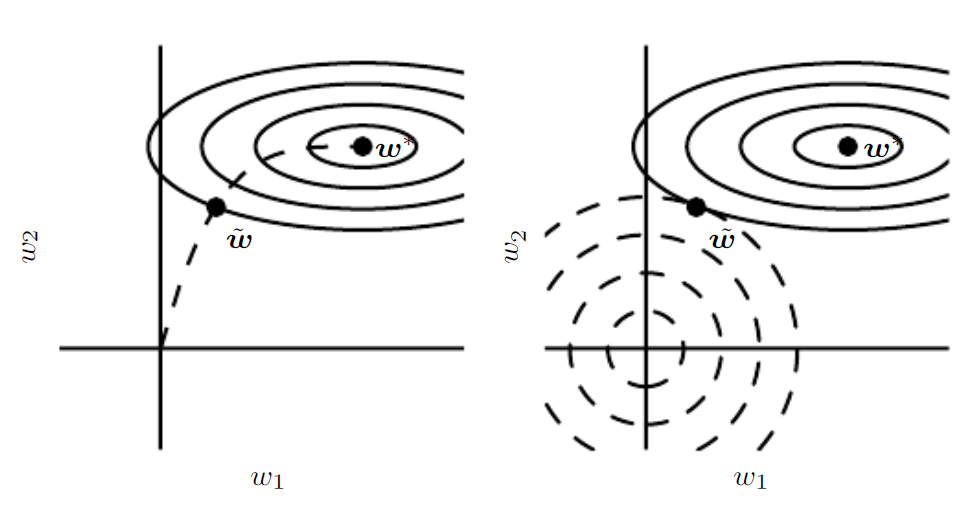
\includegraphics[height=10em]{figures/early-stop-act-as-regularization.png}
			\end{figure}
		\end{itemize}
	\end{frame}
	
	\begin{frame}{Early Stopping}
		\begin{itemize}
			\item In order to compare with classical $L^2$ regularization, we examine a simple setting where the only parameters are linear weights ($\bm{\theta}=\bm{w}$). 
			\pause
			\item We can model the cost function $J$ with a quadratic approximation in the neighborhood of the empirically optimal value of the weights $\bm{w}^*$:
			$$\hat{J}(\bm{\theta})=J(\bm{w}^*)+\frac{1}{2}(\bm{w}-\bm{w}^*)^T\bm{H}(\bm{w}-\bm{w}^*)$$
			where $\bm{H}$ is Hessian matrix of $J$ with respect to $\bm{w}$ evaluated at $\bm{w}^*$.
			\pause
			\item Given the assumption that $\bm{w}^*$ is a minimum of $J(\bm{w})$, we know that $\bm{H}$ is positive semidefinite.
		\end{itemize}
	\end{frame}
	
	\begin{frame}{Early Stopping}
		\begin{itemize}
			\item Under a local Taylor series approximation, the gradient:
			$$\nabla_{\bm{w}}\hat{J}(\bm{w})=\bm{H}(\bm{w}-\bm{w}^*)$$
			
			\pause
			\item We are going to study the trajectory followed by the parameter vector during training.
			\pause
			\item For simplicity, let us set the initial parameter vector to the origin, that is $\bm{w}^{(0)}=\bm{0}$.
			\pause
			\item Let us suppose that we update the parameters via gradient descent:
			\begin{eqnarray*}
				\bm{w}^{(\tau)}&=&\bm{w}^{(\tau-1)}-\epsilon\nabla_{\bm{w}}J(\bm{w}^{(\tau-1)})\\
				&=&\bm{w}^{(\tau-1)}-\epsilon\bm{H}(\bm{w}^{(\tau-1)}-\bm{w}^*)\\
				\bm{w}^{(\tau)}-\bm{w}^*&=&(\bm{I}-\epsilon\bm{H})(\bm{w}^{(\tau-1)}-\bm{w}^*)
			\end{eqnarray*}
		\end{itemize}
	\end{frame}
	
	\begin{frame}{Early Stopping}
		\begin{itemize}
			\item Let us now rewrite this expression in the space of the eigenvectors of $\bm{H}$, exploiting the eigendecomposition of $\bm{H}: \bm{H}=\bm{Q\Lambda Q}^T$, where $\bm{\Lambda}$ is a diagonal matrix and $\bm{Q}$ is an orthonormal basis of eigenvectors.
			\begin{eqnarray*}
				\bm{w}^{(\tau)}-\bm{w}^*&=&(\bm{I}-\epsilon\bm{Q\Lambda Q}^T)(\bm{w}^{(\tau-1)}-\bm{w}^*)\\
				\bm{Q}^T(\bm{w}^{(\tau)}-\bm{w}^*)&=&(\bm{I}-\epsilon\bm{\Lambda})\bm{Q}^T(\bm{w}^{(\tau-1)}-\bm{w}^*)
			\end{eqnarray*}
			
			\pause
			\item Assuming that $\bm{w}^{(0)}=0$ and that $\epsilon$ is chosen to be small enough to guarantee $|1-\epsilon\lambda_i|<1$, the parameter trajectory during training training after $\tau$ parameter updates is as follows:
			$$\bm{Q}^T\bm{w}^{(\tau)}=\left[\bm{I}-(\bm{I}-\epsilon\Lambda)^{\tau}\right]\bm{Q}^T\bm{w}^*$$
		\end{itemize}
	\end{frame}
	
	\begin{frame}{Early Stopping}
		\begin{itemize}
			\item In $L^2$ regularization:
			\begin{eqnarray}
				\tilde{\bm{w}}&=&\bm{Q}(\bm{\Lambda+\alpha\bm{I}})^{-1}\bm{\Lambda Q}^T\bm{w}^*\\
				\bm{Q}^T\tilde{\bm{w}}&=&(\Lambda+\alpha\bm{I})^{-1}\Lambda\bm{Q}^T\bm{w}^*\\
				\bm{Q}^T\tilde{\bm{w}}&=&\left[\bm{I}-(\bm{\Lambda}+\alpha\bm{I})^{-1}\alpha\right]\bm{Q}^T\bm{w}^*
			\end{eqnarray}
			
			\pause
			\item Compare with $\bm{Q}^T\bm{w}^{(\tau)}=\left[\bm{I}-(\bm{I}-\epsilon\Lambda)^{\tau}\right]\bm{Q}^T\bm{w}^*$, we can find:
			$$(\bm{I}-\epsilon\Lambda)^\tau=(\Lambda+\alpha\bm{I})^{-1}\alpha$$
			
			\pause
			\item Then $L^2$ regularization and early stopping is equivalent. 
			\pause
			\item Going even further, by taking logarithms and using the series expansion for $\log(1+x)$, if all $\lambda_i$ are small then:
			\begin{eqnarray}
				\tau\approx\frac{1}{\epsilon\alpha}\text{\quad;\quad}\alpha\approx\frac{1}{\tau\epsilon}
			\end{eqnarray}
			
			\pause
			\item That is, under these assumptions, the number of training iterations $\tau$ plays a role inversely proportional to the $L^2$ regularization parameter, and the inverse of $\tau\epsilon$ plays the role of the weight decay coefficient.
		\end{itemize}
	\end{frame}
	
	\begin{frame}{Parameter Tying and Parameter Sharing}
		\begin{itemize}
			\pause
			\item Thus far, we have discussed adding constraints or penalties to the parameters.
			\pause
			\item However, sometimes we may need other ways to express our \text{prior knowledge} about suitable values of the model parameters.
			\pause
			\item Sometimes we might not know precisely what values that parameters should take but we know, from knowledge of the domain and model architecture, that there should be some dependencies between the model parameters.
			\pause
			\item A common type of dependency that we often want to express is that certain parameters should be close to one another.
		\end{itemize}
	\end{frame}
	
	
	\begin{frame}{Parameter Tying and Parameter Sharing}
		Consider the following scenario:
		\begin{itemize}
			\pause
			\item We have two models performing the same classification task.
			\pause
			\item But with somewhat different input distributions.
			\pause
			\item Formally, we have model A with parameters $\bm{w}^{(A)}$ and model B with parameters $\bm{w}^{(B)}$.
			\pause
			\item The two models map the input to different, but related outputs: $\hat{y}^{(A)}=f(\bm{w}^{(A)},\bm{x})$ and $\hat{y}^{(B)}=g(\bm{w}^{(B)}, \bm{x})$.
		\end{itemize}
	\end{frame}
	
	\begin{frame}{Parameter Tying and Parameter Sharing}
		\begin{itemize}
			\item Let us imagine that the tasks are similar enough (perhaps with similar input and output distributions) that we believe the model parameters should be close to each other: $\forall i,w_i^{(A)}$ should be close to $w_i^{(B)}$. We can leverage this information through regularization.
			\pause
			\item Specifically, we can use a parameter norm penalty of the form: $\Omega(\bm{w}^{(A)}, \bm{w}^{(B)})=\lVert\bm{w}^{(A)}-\bm{w}^{(B)}\rVert^2_2$. Here we used an $L^2$ penalty, but other choices are also possible.
		\end{itemize}
	\end{frame}
	
	\begin{frame}{Parameter Tying and Parameter Sharing}
		\begin{itemize}
			\item This kind of approach was proposed by \citet{lasserre2006principled}, who regularized the parameters of one model, trained as a classifier in a supervised paradigm, to be close to the parameters of another model, trained in an unsupervised paradigm (to capture the distribution of the observed input data).
			\pause
			\item The architectures were constructed such that many of the parameters in the classifier model could paired to corresponding parameters in the unsupervised model.
		\end{itemize}
	\end{frame}
	
	\begin{frame}{Parameter Tying and Parameter Sharing}
		\begin{itemize}
			\item While a parameter norm penalty is one way to regularize parameters to be close to one another, the more popular way is to use constraints: \textbf{to force sets of parameters to be equal}. 
			\pause
			\item This method of regularization is often referred to as \emph{parameter sharing}, where we interpret the various models or model components as sharing a unique set of parameters.
			\pause
			\item A significant advantage of parameter sharing over regularizing the parameters to be close (via a norm penalty) is that only a subset of the parameters need to be stored in memory.
			\pause
			\item In certain models- such as the Convolutional Neural Network -- this can lead to significant reduction in the memory footprint of the model.
		\end{itemize}
	\end{frame}
	
	\begin{frame}{Parameter Tying and Parameter Sharing\\ Convolutional Neural Networks}
		\begin{itemize}
			\pause
			\item By far the most popular and extensive use of parameter sharing occurs in \emph{convolutional neural networks} (CNNs) applied to computer vision.
			\pause
			\item Natural images have many statistical properties that are invariant to translation.
			\pause
			\item CNNs take this property into account by sharing parameters across multiple image locations.
			\pause
			\item The same feature (a hidden unit with the same weights) is computed over different locations in the input. 
			\pause
			\item This means that we can find a object with the same object detector whether the object appears at column $i$ or column $i+1$ in the image.
			\pause
			\item Parameter sharing has allowed CNNs to dramatically lower the number of unique model parameters and to significantly increase network sizes without requiring a corresponding increase in training data.
		\end{itemize}
	\end{frame}

	\begin{frame}{Sparse Representation}
		\begin{itemize}
			\pause
			\item Weight decay acts by placing a penalty directly on the model parameters.
			\pause
			\item Another strategy is to place a penalty on the activations of the units in a neural network, encouraging their activations to be sparse.
			\pause
			\item This indirectly imposes a complicated penalty on the model parameters.
		\end{itemize}
	\end{frame}
	
	\begin{frame}{Sparse Representation}
		\begin{itemize}
			\item We have already discussed how $L^1$ penalization induces a sparse parametrization -- meaning that many of the parameters become zero (or close to zero).
			\pause
			\item Representational sparsity, on the other hand, describes a representation where many of the elements of the representation are zero (or close to zero).
		\end{itemize}
	\end{frame}
	
	\begin{frame}{Sparse Representation}
		\begin{itemize}
			\item A simplified view of this distinction can be illustrated in the context of linear regression:
			\pause
			\begin{align*}
			\underset{\bm{y} ~\in~ \mathbb{R}^m}{
				\begin{bmatrix}
				18 \\  5 \\ 15 \\ -9 \\ -3
				\end{bmatrix}} = 
			\underset{\mathbf{A} ~\in~ \mathbb{R}^{m \times n}}{
				\begin{bmatrix}
				4 & 0 & 0 & -2 & 0 & 0 \\
				0 & 0 & -1 & 0 & 3 & 0 \\
				0 & 5 & 0 & 0 & 0 & 0 \\
				1 & 0 & 0 & -1 & 0 & -4 \\
				1 & 0 & 0 & 0 & -5 & 0
				\end{bmatrix}} 
			\underset{\bm{x} ~\in~ \mathbb{R}^n}{
				\begin{bmatrix}
				2 \\ 3\\ -2\\ -5 \\ 1 \\ 4
				\end{bmatrix} }\\
			\underset{\bm{y} ~\in~ \mathbb{R}^m}{
				\begin{bmatrix}
				-14 \\  1 \\ 19 \\  2 \\ 23
				\end{bmatrix}} = 
			\underset{\mathbf{B} ~\in~ \mathbb{R}^{m \times n}}{
				\begin{bmatrix}
				3 & -1 & 2 & -5 & 4 & 1 \\
				4 & 2 & -3 & -1 & 1 & 3 \\
				-1 & 5 & 4 & 2 & -3 & -2 \\
				3 & 1 & 2 & -3 & 0 & -3 \\
				-5 & 4 & -2 & 2 & -5 & -1
				\end{bmatrix}} 
			\underset{\bm{h} ~\in~ \mathbb{R}^n}{
				\begin{bmatrix}
				0 \\ 2 \\ 0 \\ 0 \\ -3 \\ 0
				\end{bmatrix} }
			\end{align*}
		\end{itemize}
	\end{frame}
	
	\begin{frame}{Sparse Representation}
		\begin{itemize}
			\item Representational regularization is accomplished by the same sorts of mechanisms that we have used in parameter regularization.
			\pause			
			\item Norm penalty regularization of representation is performed by adding to the loss function $J$ a norm penalty on the \textbf{representation}. This penalty is denoted $\Omega(\bm{h})$. As before, we denote the regularized loss function by $\tilde{J}$:
			$$\tilde{J}(\bm{\theta};\bm{X},\bm{y})=J(\bm{\theta};\bm{X},\bm{y})+\alpha\Omega(\bm{h})$$
			
			\pause
			\item Just as an $L^1$ penalty on the parameters induces parameter sparsity, an $L^1$ penalty on the elements of the representation induces representational sparsity:
			$$\Omega(\bm{h})=\lVert\bm{h}\rVert_1=\sum_i\left|h_i\right|$$
		\end{itemize}
	\end{frame}
	
	\begin{frame}{Sparse Representation}
		\begin{itemize}
			\item Of course, the $L^1$ penalty is only one choice of penalty that can result in a sparse representation.
			\pause
			\item Others include the penalty derived from a Student-t prior on the representation (\citet{olshausen2005close,bergstra2011algorithms}) and KL divergence penalties (\citet{larochelle2008classification}) that are especially useful for representations with elements constrained to lie on the unit interval.
			\pause
			\item \citet{lee2008sparse} and \citet{goodfellow2009measuring} both provide examples of strategies based on regularizing the average activation across several examples, $\frac{1}{m}\sum_i\bm{h}^{(i)}$, to be near some target value, such as a vector with 0.01 for each entry.
		\end{itemize}
	\end{frame}
	
	\begin{frame}{Sparse Representation}
		\begin{itemize}
			\item Other approaches obtain representational sparsity with a hard constraint on the activation values.
			\pause
			\item For example, \emph{orthogonal matching pursuit} (\citet{pati1993orthogonal}) encodes an input $\bm{x}$ with representation $\bm{h}$ that solves the constrained optimization problem
			$$\mathop{\arg\min}_{\bm{h},\lVert\bm{h}\rVert_0<k}\lVert\bm{x}-\bm{Wh}\rVert^2$$
			where $\lVert\bm{h}\rVert_0$ is the number of non-zero entries of $\bm{h}$. 
			
			\pause
			\item This problem can be solved efficiently when $\bm{W}$ is constrained to be orthogonal.
			\pause
			\item This method is often called OMP-$k$ with the value of $k$ specified to indicate the number of non-zero features allowed.
			\pause
			\item \citet{coates2010analysis} demonstrated that OMP-1 can be very a effective feature extractor for deep architectures.
		\end{itemize}
	\end{frame}
	
	\begin{frame}{Bagging and Other Ensemble Methods}
		\begin{itemize}
			\pause
			\item Bagging(short for boostrap aggregating) is a technique for reducing generalization error by combining several models (\citet{breiman1996bagging}).
			\pause
			\item The idea is to train several different models separately, then have all of the models vote on the output for test examples.
			\pause
			\item This is an example of a general strategy in machine learning called \emph{model averaging}.
			\pause
			\item Techniques employing this strategy are known as \emph{ensemble methods}.
		\end{itemize}
	\end{frame}
	
	\begin{frame}{Bagging and Other Ensemble Methods}
		\begin{itemize}
			\item The reason that model averaging works is that different models will usually not make all the same errors on the test set.
			\pause
			\item Consider for example a set of $k$ regression models. 
			\pause
			\item Suppose that each model makes an error $\epsilon_i$ on each example, with the errors drawn from a zero-mean multivariate normal distribution with variance $\mathbb{E}[\epsilon_u^2]=v$ and covariance $\mathbb{E}[\epsilon_i\epsilon_j]=c$.
			\pause
			\item Then the error made by the average prediction of all the ensemble models is $\frac{1}{k}\sum_i\epsilon_i$.
			\pause
			\item The expected squared error of the ensemble predictor is
			$$\mathbb{E}\left[\left(\frac{1}{k}\sum_i\epsilon_i\right)^2\right]=\frac{1}{k^2}\mathbb{E}\left[\sum_i\left(\epsilon_i^2+\sum_{i\neq j}\epsilon_i\epsilon_j\right)\right]=\frac{1}{k}v+\frac{k-1}{k}c$$
		\end{itemize}
	\end{frame}
	
	\begin{frame}{Bagging and Other Ensemble Methods}
		$$\mathbb{E}\left[\left(\frac{1}{k}\sum_i\epsilon_i\right)^2\right]=\frac{1}{k}v+\frac{k-1}{k}c$$
		\begin{itemize}
			\item In the case where the errors are perfectly correlated and $c=v$, the mean squared error reduces to $v$, so the model average does not help at all.
			\pause
			\item In the case where the errors are perfectly uncorrelated and $c=0$, the expected squared error of the ensemble is only $\frac{1}{k}v$. This means that the expected squared error of the ensemble decreases linearly with the ensemble size.
			\pause
			\item In other words, on average, the ensemble will perform at least as well as any of its members, and if the members make independent errors, the ensemble will perform significantly better than it members.
		\end{itemize}
	\end{frame}
	
	\begin{frame}{Bagging and Other Ensemble Methods}
		\begin{itemize}
			\item Different ensemble methods construct the ensemble of the models in different ways.
			\pause
			\item For example, each member of the ensemble could be formed by training a completely different kind of model using a different algorithm or objective function.
			\pause
			\item Bagging is a method that allows the same kind of model, training algorithm and objective function to be reused several times.
			\pause
			\item Specifically, bagging involves constructing $k$ different datasets.
			\pause
			\item Each dataset has the same number of examples as the original dataset, but each dataset is constructed by sampling with replacement from the origin dataset.
			\pause
			\item This means that, with high probability, each dataset is missing some of the examples from the original dataset and also contains several duplicate examples.
			\pause
			\item Model $i$ is then trained on dataset $i$.
		\end{itemize}
	\end{frame}
	
	\begin{frame}{Bagging and Other Ensemble Methods}
		\begin{figure}
			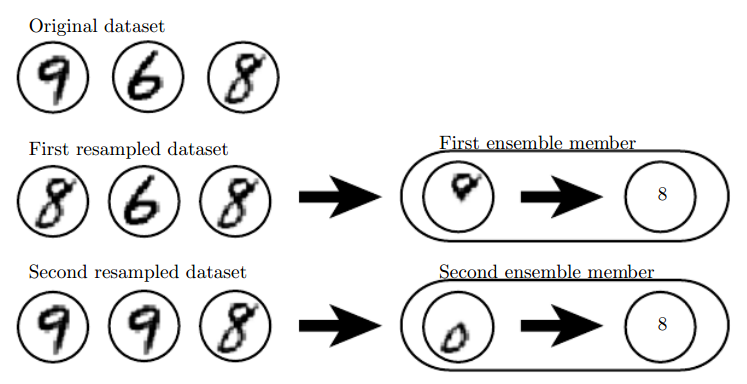
\includegraphics[height=15em]{figures/bagging.png}
			\caption{A cartoon depiction of how bagging works}
		\end{figure}
	\end{frame}
	
	\begin{frame}{Bagging and Other Ensemble Methods}
		\begin{itemize}
			\item Neural networks reach a wide enough variety of solution points that they can often benefit from model averaging even if all of the models are trained on the same dataset.
			\pause
			\item Differences in random initialization, random selection of minibatches, differences in hyperparameters, or different outcomes of non-deterministic implementations of neural networks are often enough to cause different members of the ensemble to make partially independent errors.
		\end{itemize}
	\end{frame}
	
	\begin{frame}{Bagging and Other Ensemble Methods}
		\begin{itemize}
			\item Model averaging is an extremely powerful and reliable method for reducing generalization error.
			\pause
			\item Its use is usually discouraged when benchmarking algorithms for scientific papers.
			\pause
			\item Machine learning contest are usually won by methods using model averaging over dozens of models.
			\pause
			\item Not all techniques for constructing ensembles are designed to make the ensemble more regularized than the individual models.
			\pause
			\item For example, a technique called \emph{boosting} (\citet{freund1996experiments}) constructs an ensemble with higher capacity than the individual models. 
		\end{itemize}
	\end{frame}
	
	\begin{frame}{Bagging and Other Ensemble Methods}
		\begin{itemize}
			\item Boosting has been applied to build ensembles of neural networks (\citet{schwenk1998training}) by incrementally adding neural networks to the ensemble.
			\pause
			\item Boosting has also been applied interpreting an individual neural network as an ensemble (\citet{bengio2006convex}), incrementally adding hidden units to the neural network.
		\end{itemize}
	\end{frame}
	
	\begin{frame}{Dropout}
		\begin{itemize}
			\pause
			\item Dropout (\citep{srivastava2014dropout}) provides a computationally inexpensive but powerful method of regularizing a broad family of models.
			\pause
			\item Dropout can be thought of as a method of making bagging practical for ensembles of very many large neural networks.
			\pause
			\item Bagging involves training multiple models, and evaluating multiple models on each test example. 
			\pause 
			\item This seems impractical when each model is a large neural network, since training and evaluating such networks is costly in terms of runtime and memory.
			\pause
			\item It is common to use ensembles of five to ten neural networks. but more than this rapidly becomes unwieldy.
			\pause
			\item Dropout provides an inexpensive approximation to training and evaluating a bagged ensemble of exponentially many neural networks.
		\end{itemize}
	\end{frame}
	
	\begin{frame}{Dropout}
		Specifically, dropout trains the ensemble consisting of all sub-networks that can be formed by removing non-output units from an underlying base network.
		\begin{columns}
			\column{0.6\textwidth}
			\begin{itemize}
				\item In the most modern neural networks, based on a series of affine transformations and nonlinearities, we can effectively remove a unit from a network by multiplying its output value by zero. 
				\item This procedure requires some slight modification for models such as radial basis function networks, which take the difference between the unit's state and some reference value.
			\end{itemize}
			\column{0.4\textwidth}
			\begin{figure}
				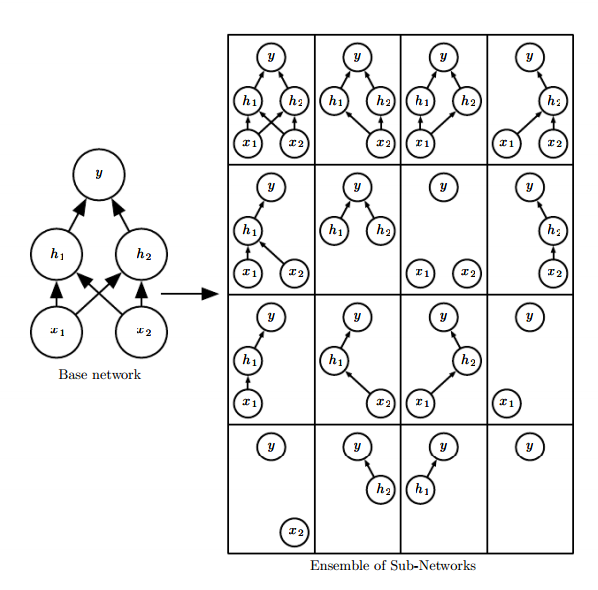
\includegraphics[height=13em]{figures/dropout.png}
			\end{figure}
		\end{columns}
	\end{frame}
	
	\begin{frame}{Dropout}
		\begin{itemize}
			\item Here, we present the dropout algorithm in terms of multiplication by zero for simplicity, but it can be trivially modified to work with other operations that remove a unit from the network.
			\pause
			\item Recall that to learn with bagging, we define $k$ different models, construct $k$ different datasets by sampling from the training set with replacement, and then train model $i$ on dataset $i$.
			\pause
			\item Dropout aims to approximate this process, but with an exponentially large number of neural networks.
		\end{itemize}
	\end{frame}
	
	\begin{frame}{Dropout}
		\begin{itemize}
			\item Specifically, to train with dropout, we use a minibatch-based learning algorithm that makes small steps, such as stochastic gradient descent.
			\pause
			\item Each time we load an example into a minibatch, we randomly sample a different binary mask to apply to all of the input and hidden units in the network.
			\pause
			\item The mask for each unit is sampled independently from all of the others. 
			\pause
			\item The probability of sampling a mask value of one is a hyperparameter fixed before training begins.
			\pause
			\item Typically, an input unit is included with probability 0.8 and a hidden unit is included with probability 0.5.
			\pause
			\item We then run forward propagation, back-propagation, and the learning update as usual.
		\end{itemize}
	\end{frame}
	
	\begin{frame}{Dropout}
		\begin{columns}
			\column{0.5\textwidth}
			\begin{figure}
				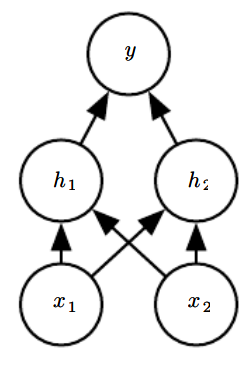
\includegraphics[height=12em]{figures/dropout-computation-graph-1.png}
			\end{figure}
			\column{0.5\textwidth}
			\begin{figure}
				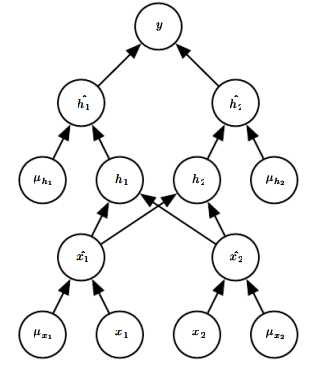
\includegraphics[height=17em]{figures/dropout-computation-graph-2.png}
			\end{figure}
		\end{columns}
	\end{frame}
	
	\begin{frame}{Dropout}
		\begin{itemize}
			\item More formally, suppose that a mask vector $\mu$ specifies which units to include, and $\bm{J}(\bm{\theta},\bm{\mu})$ defines the cost of the model defined by parameters $\bm{\theta}$ and mask $\bm{\mu}$.
			\pause
			\item Then dropout training consists in minimizing $\mathbb{E}_{\bm{\mu}}\bm{J}(\bm{\theta},\bm{\mu})$.
			\pause
			\item The expectation contains exponentially many terms but we can obtain an unbiased estimate of its gradient by sampling values of $\mu$
		\end{itemize}
	\end{frame}
	
	\begin{frame}{Dropout}
		\begin{itemize}
			\item Dropout training is not quite the same as bagging traing.
			\pause
			\item In the case of bagging, the models are all independent.
			\pause
			\item In the case of dropout, the models share parameters, with each model inheriting a different subset of parameters from the parent neural network. This parameter sharing makes it possible to represent an exponential number of models with a tractable amount of memory.
			\pause
			\item In the case of bagging, each model is trained to convergence on its respective training set.
		\end{itemize}
	\end{frame}
	
	\begin{frame}{Dropout}
		\begin{itemize}
			\item In the case of dropout, typically most models are not explicitly trained at all--usually, the model is large enough that it would be infeasible to sample all possible subnetworks within the lifetime of the universe.
			\pause
			\item Instead, a tiny fraction of the possible sub-networks are each trained for a single step, and the parameter sharing causes the remaining sub-networks to arrive at good settings of the parameters.
			\pause
			\item Beyond these, dropout follows the bagging algorithm.
		\end{itemize}
	\end{frame}
	
	\begin{frame}{Dropout}
		\begin{itemize}
			\item To make a prediction, a bagged ensemble must accumulate votes from all of its members. We refer to this process as \emph{inference} in this context.
			\pause
			\item Now, we assume that the model's role is to output a probability distribution.
			\pause
			\item In the case of bagging, each model $i$ produces a probability distribution $p^{(i)}(y|\bm{x})$. 
			\pause
			\item The prediction of the ensemble is given by the arithmetic mean of all of these distributions
			$$\frac{1}{k}\sum_{i=1}^kp^{(i)}(y|\bm{x})$$			
		\end{itemize}
	\end{frame}
	
	\begin{frame}{Dropout}
		\begin{itemize}
			\item In the case of dropout, each sub-model defined by mask vector $\bm{\mu}$ defines a probability distribution $p(y|\bm{x},\bm{\mu})$.
			\pause
			\item The arithmetic mean over all masks is given by
			$$\sum_{\bm{\mu}} p(\bm{\mu})p(y|\bm{x},\bm{\mu})$$
			
			where $p(\bm{\mu})$ is the probability distribution that was used to sample $\mu$ at training time.
			\pause
			\item Because this sum includes an exponential number of terms, it is intractable to evaluate except in cases where the structure of the model permits some form of simplification.
			\pause
			\item We can approximate the inference with sampling, by averaging together the output from many masks.
		\end{itemize}
	\end{frame}
	
	\begin{frame}{Dropout}
		\begin{itemize}
			\item However, there is an even better approach, that allows us to obtain a good approximation to the predictions of the entire ensemble, at the cost of only one forward propagation.
			\pause
			\item To do so, we change to using the geometric mean rather than the arithmetic mean of the ensemble member's prediction distributions.
			\pause
			\item \citet{warde2013empirical} present arguments and empirical evidence that the geometric mean performs comparably to the arithmetic mean in this context.
		\end{itemize}
	\end{frame}
	
	\begin{frame}{Dropout}
		\begin{itemize}
			\item The geometric mean of multiple probability distributions is not guaranteed to be a probability distribution.
			\pause
			\item To guarantee that the result is a probability distribution, we impose the requirement that none of the sub-models assigns probability 0 to any event, and we renormalize the resulting distribution.
			\pause
			\item The unnormalized probability distribution defined directly by the geometric mean is given by
			$$\tilde{p}_{\text{ensemble}}(y|\bm{x})=\sqrt[2^d]{\prod_{\bm{\mu}}p(y|\bm{x},\bm{\mu})}$$
			
			where $d$ is the number of units that may be dropped.
		\end{itemize}
	\end{frame}
	
	\begin{frame}{Dropout}
		\begin{itemize}
			\item Here we use a uniform distribution over $\bm{\mu}$ to simplify the presentation, but non-uniform distributions are also possible.
			\pause
			\item To make predictions we must re-normalize the ensemble:
			$$p_{\text{ensemble}}(y|\bm{x})=\frac{\tilde{p}_{\text{ensemble}}(y|\bm{x})}{\sum_{y'}\tilde{p}_{\text{ensemble}}(y'|\bm{x})}$$
			
			\pause
			\item The key insight (\citet{hinton2012improving}) involved in dropout is that we can approximate $p_{\text{ensemble}}$ by evaluating $p(y|\bm{x})$ in one model: the model with all units, but with the weight going out of unit $i$ multiplied by the probability of including unit $i$.
			\pause
			
			\item We call this approach the \emph{weight scaling inference rule}.
			\pause
			\item There is not yet any theoretical argument for the accuracy of this approximate inference rule in deep nonlinear networks, but empirically it performs very well.
		\end{itemize}
	\end{frame}
	
	\begin{frame}{Dropout}
		\begin{itemize}
			\item Because we usually use an inclusion probability of $\frac{1}{2}$, the weight scaling rule usually amounts to dividing the weights by 2 at the end of training, and then using the model as usual.
			\pause
			\item Another way to achieve the same result is to multiply the states of the units by 2 during training.
			\pause
			\item Either way, the goal is to make sure that the expected total input to a unit at test time is roughly the same as the expected total input to that unit at train time, even though half the units at train time are missing on average.
		\end{itemize}
	\end{frame}
	
	\begin{frame}{Dropout}
		\begin{itemize}
			\item For many classes of models that do not have nonlinear hidden units, the weight scaling inference rule is exact.
			\pause
			\item For a simple example, consider a softmax regression classifier with $n$ input variables represented by the vector $\bm{\mathrm{v}}$:
			$$P(\mathrm{y}=y|\bm{\mathrm{v}})=\mathrm{softmax}(\bm{\mathrm{W}}^T\bm{\mathrm{v}}+\bm{b})_y$$
			
			\pause
			\item We can index into the family of sub-models by element-wise multiplication of the input with a binary vector $d$:
			$$P(\mathrm{y}=y|\bm{\mathrm{v}};\bm{d})=\mathrm{softmax}(\bm{\mathrm{W}}^T(\bm{d}\odot\bm{\mathrm{v}})+\bm{b})_y$$
		\end{itemize}
	\end{frame}
	
	\begin{frame}{Dropout}
		\begin{itemize}
			\item The ensemble predictor is defined by re-normalizing the geometric mean over all ensemble members' predictions
			$$P_{\text{ensemble}}(\mathrm{y}=y|\bm{\mathrm{v}})=\frac{\tilde{P}_{\text{ensemble}}(\mathrm{y}=y|\bm{\mathrm{v}})}{\sum_{y'}\tilde{P}_{\text{ensemble}}(\mathrm{y}=y'|\bm{v})}$$
			
			where
			$$\tilde{P}_{\text{ensemble}}(\mathrm{y}=y|\bm{v})=\sqrt[2^n]{\prod_{\bm{d}\in\{0,1\}^n}P(\mathrm{y}=y|\bm{\mathrm{v}};\bm{d})}$$
		\end{itemize}
	\end{frame}
	
	\begin{frame}{Dropout}
		\begin{itemize}
			\item To see that the weight scaling rule is exact, we can simplify 
			\pause
			\begin{eqnarray*}
				\tilde{P}_{\text{ensemble}}\left(\mathrm{y}=y|\bm{\mathrm{v}}\right)&=&\sqrt[2^n]{\prod_{\bm{d}\in\{0,1\}^n}P\left(\mathrm{y}=y|\bm{\mathrm{v}};\bm{d}\right)}\\
				&=&\sqrt[2^n]{\prod_{\bm{d}\in\{0,1\}^n}\text{softmax}\left(\bm{\mathrm{W}}^T(\bm{d}\odot\bm{\mathrm{v}})+\bm{b}\right)_y}\\
				&=&\sqrt[2^n]{\prod_{\bm{d}\in\{0,1\}^n}\frac{\exp\left(\bm{\mathrm{W}}^T_{y,:}\left(\bm{d}\odot\bm{\mathrm{v}}\right)+\bm{b}\right)}{\sum_{y'}\exp\left(\bm{\mathrm{W}}^T_{y',:}\left(\bm{d}\odot\bm{\mathrm{v}}\right)+\bm{b}\right)}}\\
				&=&\frac{\sqrt[2^n]{\prod_{\bm{d}\in\{0,1\}^n}\exp\left(\bm{\mathrm{W}}^T_{y,:}\left(\bm{d}\odot\bm{\mathrm{v}}\right)+\bm{b}\right)}}{\sqrt[2^n]{\prod_{\bm{d}\in\{0,1\}^n}\sum_{y'}\exp\left(\bm{\mathrm{W}}^T_{y',:}\left(\bm{d}\odot\bm{\mathrm{v}}\right)+\bm{b}\right)}}
			\end{eqnarray*}
		\end{itemize}
	\end{frame}
	
	\begin{frame}{Dropout}
		\begin{itemize}
			\item Because $\tilde{P}$ will be normalized, we can safely ignore multiplication by factors that are constant with respect to $y$:
			\pause
			\begin{eqnarray*}
				\tilde{P}_{\text{ensemble}}(\mathrm{y}=y|\bm{\mathrm{v}})&\propto&\sqrt[2^n]{\prod_{\bm{d}\in\{0,1\}^n}\exp\left(\bm{\mathrm{W}}^T_{y,:}\left(\bm{d}\odot\bm{\mathrm{v}}\right)+\bm{b}\right)}\\
				&=&\exp\left(\frac{1}{2^n}\sum_{\bm{d}\in\{0,1\}^n}\bm{\mathrm{W}}^T_{y,:}\left(\bm{d}\odot\bm{\mathrm{v}}\right)+\bm{b}\right)\\
				&=&\exp\left(\frac{1}{2}\bm{\mathrm{W}}^T_{y,:}\bm{\mathrm{v}}+\bm{b}\right)
			\end{eqnarray*}
			\pause
			\item Substituting this back into $P_{\text{ensemble}}(\mathrm{y}=y|\bm{\mathrm{v}})=\frac{\tilde{P}_{\text{ensemble}}(\mathrm{y}=y|\bm{\mathrm{v}})}{\sum_{y'}\tilde{P}_{\text{ensemble}}(\mathrm{y}=y'|\bm{v})}$ we obtain a softmax classifier with weights $\frac{1}{2}\bm{\mathrm{W}}$
		\end{itemize}
	\end{frame}
	
	\begin{frame}{Dropout}
		\begin{itemize}
			\item The weight scaling rule is also exact in other settings, including regression networks with conditionally normal outputs, and deep networks that have hidden layers without nonlinearities.
			\pause
			\item However, the weight scaling rule is only a approximation for deep models that have nonlinearities.
			\pause
			\item Though the approximation has not been theoretically characterized, it often works well, empirically.
			\pause
			\item \citet{goodfellow2013maxout} found experimentally that the weight scaling approximation can work better (in terms of classification accuracy) than Monte Carlo approximations to the ensemble predictor.
			\pause
			\item This held true even when the Monte Carlo approximation was allowed to sample up to 1,000 sub-networks.
		\end{itemize}
	\end{frame}
	
	\begin{frame}{Dropout}
		\begin{itemize}
			\item \citet{gal2015bayesian} found that some models obtain better classification accuracy using twenty samples and the Monte Carlo approximation. It appears that the optimal choice of inference approximation is problem-depend.
			\pause
			\item \citet{srivastava2014dropout} showed that dropout is more effective than other standard computationally inexpensive regularizers, such as weight decay, filter norm constraints and sparse activity regularization.
			\pause
			\item One advantage of dropout is that it is very computationally cheap.
			\pause
			\item Another significant advantage of dropout is that it does not significantly limit the type of model or training procedure that can be used.
			\pause
			\item This includes feedforward neural networks, probabilistic models such as restricted Boltzmann machines (\citet{srivastava2014dropout}), and recurrent neural networks (\citet{bayer2014learning,pascanu2013construct}).
		\end{itemize}
	\end{frame}
	
	\begin{frame}{Dropout}
		\begin{itemize}
			\item \citet{wager2013dropout} showed that, when applied to linear regression, dropout is equivalent to $L^2$ weight decay, with a different weight decay coefficient for each input feature.
			\pause
			\item The magnitude of each feature's weight decay coefficient is determined by its variance.
			\pause
			\item Similar results hold for other linear models.
			\pause
			\item For deep models, dropout is not equivalent to weight decay.
		\end{itemize}
	\end{frame}
	
	\begin{frame}{Dropout}
		\begin{itemize}
			\item The power of dropout arises from the fact that the masking noise is applied to the hidden units.
			\pause
			\item This can be seen as a form of highly intelligent, adaptive destruction of the information content of the input rather than destruction of the raw values of the input.
			\pause
			\item For example, if the model learns a hidden unit $h_i$ that detects a face by finding the nose, then dropping $h_i$ corresponds to erasing the information that there is a nose in the image.
			\pause
			\item The model must learn another $h_i$, either that redundantly encodes the presence of a nose, or that detects the face by another feature, such as the mouth.
			\pause
			\item Destroying extracted features rather than original values allows the destruction process to make use of all of the knowledge about the input distribution that the model has acquired so far.
		\end{itemize}
	\end{frame}
	
	\begin{frame}{Adversarial Training}
		\begin{itemize}
			\pause
			\item Im many cases, neural networks have begun to reach human performance when evaluated on an i.i.d. test set. It is natural therefore to wonder whether these models have obtained a true human-level understanding of these tasks.
			\pause
			\item In order to probe the level of understanding a network has of the underlying task, we can search for examples that the models misclassifies.
			\pause
			\item \citet{szegedy2013intriguing} found that even neural networks that perform at human level accuracy have a nearly 100\% error rate on examples that are intentionally constructed by using an optimization procedure to search for an input $\bm{x'}$ near a data point $\bm{x}$ such that the model output is very different at $\bm{x'}$
			\pause
			\item In many cases, $\bm{x'}$ can be so similar to $\bm{x'}$ that a human observer cannot tell the difference between the original example and the \emph{adversarial example}, but the network can make highly different predictions.
		\end{itemize}
	\end{frame}
	
	\begin{frame}{Adversarial Training}
		\begin{figure}
			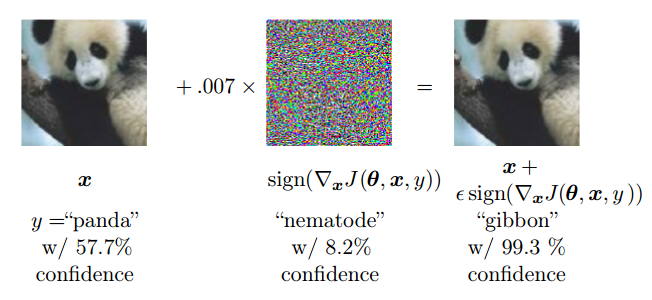
\includegraphics[height=15em]{figures/adversarial-example.png}
		\end{figure}
	\end{frame}
	
	\begin{frame}{Adversarial Training}
		\begin{itemize}
			\item Adversarial examples are interesting in the context of regularization because one can reduce the error rate on the original i.i.d. test set via \emph{adversarial training}-- training on adversarially perturbed examples from from the training set.
			\pause
			\item \citet{goodfellow2013multi} showed that one of the primary causes of these adversarial examples is excessive linearity.
			\pause
			\item Neural networks are built out of primarily linear building blocks.
			\pause
			\item In some experiments the overall function they implement proves to be highly linear as a result.
			\pause
			\item Unfortunately, the value of a linear function can change very rapidly if it has numerous inputs.
			\pause
			\item If we change each input by $\epsilon$, then a linear function with weights $\bm{w}$ can change by as much as $\epsilon\lVert\bm{w}\rVert_1$, which can be a very large amount if $\bm{w}$ is high-dimensional.
		\end{itemize}
	\end{frame}
	
	\begin{frame}{Adversarial Training}
		\begin{itemize}
			\item Adversarial training discourages this highly sensitive locally linear behavior by encouraging the network to be locally constant in the neighborhood of the training data.
			\pause
			\item This can be seen as a way of explicitly introducing a local constancy prior into supervised neural networks.
		\end{itemize}
	\end{frame}
	
	\begin{frame}{Adversarial Training}
		\begin{itemize}
			\item Adversarial training helps to illustrate the power of using a large function family in combination with aggressive regularization.
			\pause
			\item Purely linear models, like logistic regression, are not able to resist adversarial examples because they are forced to be linear.
			\pause
			\item Neural networks are able to represent functions that can range from nearly linear to nearly locally constant and thus have the flexibility to capture linear trends in the training data while still learning to resist local perturbation.
		\end{itemize}
	\end{frame}
	
	\begin{frame}{Adversarial Training}
		\begin{itemize}
			\item Adversarial examples also provide a means of accomplishing semi-supervised learning.
			\pause
			\item At a point $\bm{x}$ that is not associated with a label in the dataset, the model itself assigns some label $\hat{y}$.
			\pause
			\item The model's label $\hat{y}$ may not be the true label, but if the model is high quality, then $\hat{y}$ has a high probability of providing the true label.
			\pause
			\item We can seek an adversarial example $\bm{x}'$ that causes the classifier to output a label $y'$ with $y'\neq\hat{y}$.
			\pause
			\item The classifier may then be trained to assign the same label to $\bm{x}$ and $\bm{x}'$.
			\pause
			\item Adversarial examples generated using not the true label but a label provided by a trained model are called \emph{virtual adversarial examples}.
			\pause
			\item This encourages the classifier to learn a function that is robust to small changes.
		\end{itemize}
	\end{frame}
	
	\begin{frame}{Tangent Distance, Tangent Prop, and Manifold Tangent Classifier}
		\begin{itemize}
			\item The \emph{tangent prop} algorithm (\citet{simard1991tangent}) trains a neural net classifier with an extra penalty to make each output $f(\bm{x})$ of the neural net locally invariant to known factors of variation.
			\pause
			\item The directional derivative of $f$ at $\bm{x}$ in the directions $\bm{v}^{(i)}$ be small by adding a regularization penalty $\Omega$:
			$$\Omega(f)=\sum_i\left(\left(\nabla_{\bm{x}}f(\bm{x})\right)^2\bm{v}^{(i)}\right)^2$$
		\end{itemize}
	\end{frame}
	
	
	\begin{frame}[allowframebreaks]{References}
		\bibliography{Chap7}
		\bibliographystyle{plainnat}
	\end{frame}
\end{document}
